\documentclass[aspectratio=169,11pt]{beamer}

\usepackage[T1]{fontenc}
\usepackage[utf8]{inputenc}
\usepackage[brazilian]{babel}
\usepackage{lmodern}
\usepackage{graphicx}
\usepackage{booktabs}
\usepackage{amsmath}
\usepackage{array}
\usepackage{hyperref}
\usepackage{multicol}
\usepackage{tikz}
\usepackage{pgfplots}
\pgfplotsset{compat=1.18}

% -----------------------------------------------------------------------------
% Identidade visual
% -----------------------------------------------------------------------------
\definecolor{RoxoPrincipal}{HTML}{4D4057}
\definecolor{RoxoSecundario}{HTML}{75657F}
\definecolor{MalvaDestaque}{HTML}{9A6F86}
\definecolor{LavandaClaro}{HTML}{F1EDF3}
\definecolor{LavandaLinha}{HTML}{D8CFDD}
\definecolor{CinzaTexto}{HTML}{413C43}

\usetheme{default}
\useinnertheme{rounded}
\setbeamertemplate{navigation symbols}{}

\setbeamercolor{normal text}{fg=CinzaTexto,bg=white}
\setbeamercolor{structure}{fg=RoxoPrincipal}
\setbeamercolor{title}{fg=white}
\setbeamercolor{subtitle}{fg=white}
\setbeamercolor{author}{fg=white}
\setbeamercolor{institute}{fg=white!90}
\setbeamercolor{date}{fg=white!80}
\setbeamercolor{frametitle}{fg=white,bg=RoxoPrincipal}
\setbeamercolor{block title}{fg=white,bg=RoxoSecundario}
\setbeamercolor{block body}{fg=CinzaTexto,bg=LavandaClaro}
\setbeamercolor{block title alerted}{fg=white,bg=MalvaDestaque}
\setbeamercolor{block body alerted}{fg=CinzaTexto,bg=LavandaClaro}
\setbeamercolor{alerted text}{fg=MalvaDestaque}
\setbeamercolor{footline}{fg=RoxoPrincipal,bg=white}
\setbeamercolor{footline line}{bg=LavandaLinha}

\setbeamerfont{title}{size=\LARGE,series=\bfseries}
\setbeamerfont{subtitle}{size=\large}
\setbeamerfont{frametitle}{size=\large,series=\bfseries}
\setbeamerfont{footline}{size=\scriptsize}

% Logo da UFPE com uma base clara para contraste.
\newcommand{\marcaInstitucional}[1]{%
  \begin{tikzpicture}[baseline=(marca.base)]
    \node[fill=white,rounded corners=2pt,inner sep=2.2pt] (marca) {%
      
\includegraphics[height=#1]{logo_ufpe.png}%
    };
  \end{tikzpicture}%
}

% Cabeçalho roxo com a marca institucional em todos os slides de conteúdo.
\setbeamertemplate{frametitle}{%
  \nointerlineskip
  \begin{beamercolorbox}[
    wd=\paperwidth,ht=3.4ex,dp=1.45ex,leftskip=0.58cm,rightskip=1.75cm
  ]{frametitle}%
    \usebeamerfont{frametitle}\insertframetitle
  \end{beamercolorbox}%
  \begin{tikzpicture}[remember picture,overlay]
    \node[anchor=north east,fill=white,rounded corners=2pt,inner sep=1.2pt]
      at ([xshift=-0.32cm,yshift=-0.16cm]current page.north east)
      {
\includegraphics[height=0.52cm]{logo_ufpe.png}};
  \end{tikzpicture}%
}

% Rodapé leve, com seção atual e paginação em formato de cápsula.
\setbeamertemplate{footline}{%
  \leavevmode%
  \vbox{%
    \begin{beamercolorbox}[wd=\paperwidth,ht=0.22ex,dp=0ex]{footline line}
    \end{beamercolorbox}%
    \hbox{%
      \begin{beamercolorbox}[wd=.28\paperwidth,ht=3.0ex,dp=1.15ex,leftskip=0.55cm]{footline}
        \usebeamerfont{footline}\insertshortauthor
      \end{beamercolorbox}%
      \begin{beamercolorbox}[wd=.52\paperwidth,ht=3.0ex,dp=1.15ex,center]{footline}
        \usebeamerfont{footline}\insertsectionhead
      \end{beamercolorbox}%
      \begin{beamercolorbox}[wd=.20\paperwidth,ht=3.0ex,dp=0.65ex,rightskip=0.45cm plus 1fil]{footline}
        \tikz[baseline=-0.65ex]{%
          \node[fill=RoxoPrincipal,text=white,rounded corners=5pt,
            inner xsep=7pt,inner ysep=2.3pt] {%
            \usebeamerfont{footline}\insertframenumber\,/\,\inserttotalframenumber
          };
        }%
      \end{beamercolorbox}%
    }%
  }%
  \vskip0pt%
}

% -----------------------------------------------------------------------------
% Informações editáveis da apresentação
% -----------------------------------------------------------------------------
\newcommand{\telefone}{(81) 98538-4702}
\newcommand{\email}{Romadeoliveira@hotmail.com}
\newcommand{\linkedin}{linkedin.com/in/romariojonas-veloso-427373175}
\newcommand{\portfolio}{romariojonas.com}
\newcommand{\lattes}{lattes.cnpq.br/7040983804231610}

\title[Filtro ativo MFB]{Filtro Ativo Passa-Faixa MFB}
\subtitle{Função de transferência, resposta em frequência e validação teórico-experimental}
\author[Romário J. O. Veloso]{Romário J. O. Veloso}
\institute{Bacharelando em Engenharia Eletrônica\\
Universidade Federal de Pernambuco -- UFPE\\
Centro de Tecnologia e Geociências -- CTG\\
Departamento de Eletrônica e Sistemas -- DES}
\date{20 de setembro de 2026}

\begin{document}

% Capa
{
\setbeamercolor{background canvas}{bg=RoxoPrincipal}
\setbeamertemplate{footline}{}
\begin{frame}[plain]
  \begin{center}
    \vspace{0.12cm}
    \marcaInstitucional{1.42cm}\par
    \vspace{0.36cm}
    {\usebeamerfont{title}\color{white}\inserttitle\par}
    \vspace{0.22cm}
    {\usebeamerfont{subtitle}\color{white!82}\insertsubtitle\par}
    \vspace{0.38cm}
    {\color{MalvaDestaque}\rule{0.22\textwidth}{2pt}}\par
    \vspace{0.38cm}
    {\usebeamerfont{author}\color{white}\insertauthor\par}
    \vspace{0.12cm}
    {\usebeamerfont{institute}\color{white!84}\insertinstitute\par}
    \vfill
    {\color{white!72}\small Prática 2 de Circuitos Elétricos 2\quad\textbullet\quad Recife -- Pernambuco\quad\textbullet\quad \insertdate}
  \end{center}
\end{frame}
}
% Sumário
\begin{frame}{Sumário}
  \tableofcontents[hideallsubsections]
\end{frame}

\section{Introdução}
% Introdução: contexto da prática 2
\begin{frame}{Contexto da prática}
  \begin{block}{Problema investigado}
    Determinar como a função de transferência de um filtro ativo influencia sua
    resposta em regime permanente senoidal, confrontando o modelo matemático com
    a simulação e com as medições realizadas em bancada.
  \end{block}

  \begin{columns}[T,onlytextwidth]
    \begin{column}{0.48\textwidth}
      \textbf{Grandezas observadas}
      \begin{itemize}
        \item ganho $|H(j\omega)|=V_o/V_i$;
        \item fase $\phi=360^{\circ}\,\Delta T/T$;
        \item frequência de ressonância;
        \item característica passa-faixa.
      \end{itemize}
    \end{column}
    \begin{column}{0.48\textwidth}
      \textbf{Etapas complementares}
      \begin{itemize}
        \item análise no domínio da frequência;
        \item cálculo simbólico e numérico;
        \item validação no LTspice;
        \item ensaio com protoboard e osciloscópio.
      \end{itemize}
    \end{column}
  \end{columns}
\end{frame}
% Objetivos
\begin{frame}{Objetivos}
  \begin{block}{Objetivo geral}
    Analisar a resposta em frequência de um filtro ativo de realimentação múltipla
    (MFB) e verificar a capacidade da função de transferência de prever seu
    comportamento em regime permanente senoidal.
  \end{block}

  \begin{itemize}
    \item Obter analiticamente a função de transferência $H(s)$ do circuito.
    \item Calcular magnitude e fase para frequências entre $40\,\mathrm{Hz}$ e
      $11\,\mathrm{kHz}$.
    \item Validar o modelo por cálculo simbólico e simulação no LTspice.
    \item Medir amplitudes e defasagem com o osciloscópio.
    \item Comparar teoria, simulação e experimento, identificando fontes de erro.
  \end{itemize}
\end{frame}
% Metodologia de validação
\begin{frame}{Metodologia de validação}
  \small
  \begin{columns}[T,onlytextwidth]
    \begin{column}{0.31\textwidth}
      \begin{block}{1. Análise teórica}
        \begin{itemize}
          \item aplicação da LKC;
          \item obtenção de $H(s)$;
          \item substituição $s=j\omega$;
          \item cálculo de módulo e fase.
        \end{itemize}
      \end{block}
    \end{column}
    \begin{column}{0.31\textwidth}
      \begin{block}{2. Simulação}
        \begin{itemize}
          \item circuito reproduzido no LTspice;
          \item alimentação simétrica de $\pm10\,\mathrm{V}$;
          \item senoide de $100\,\mathrm{mV}$;
          \item varredura de $40\,\mathrm{Hz}$ a $11\,\mathrm{kHz}$;
        \end{itemize}
      \end{block}
    \end{column}
    \begin{column}{0.31\textwidth}
      \begin{block}{3. Ensaio em bancada}
        \begin{itemize}
          \item montagem em protoboard;
          \item amplificador operacional e fonte simétrica;
          \item gerador e osciloscópio;
          \item conferência dos componentes;
          \item dois canais de medição;
        \end{itemize}
      \end{block}
    \end{column}
  \end{columns}

  \vspace{0.08cm}
  \begin{alertblock}{Processamento dos sinais}
    \centering
    $|H(j\omega)|=V_o/V_i$
    \qquad e \qquad
    $\phi=360^{\circ}\,\Delta T/T$.
  \end{alertblock}
\end{frame}
% Circuito ativo estudado
\begin{frame}{Filtro passa-faixa de realimentação múltipla}
  \begin{columns}[T,onlytextwidth]
    \begin{column}{0.60\textwidth}
      \centering
      \includegraphics[
        page=7,
        trim=135bp 572bp 120bp 78bp,
        clip,
        width=\linewidth,
        height=0.61\textheight,
        keepaspectratio
      ]{\detokenize{prism-uploads/Romário_Jonas_-_relatório_Pratica_02___Circuitos_Elétricos_2.pdf}}

      \vspace{0.08cm}
      \scriptsize Circuito MFB analisado.
    \end{column}
    \hfill
    \begin{column}{0.36\textwidth}
      \small
      \begin{block}{Topologia}
        Filtro ativo passa-faixa de segunda ordem, com amplificador operacional e
        duas malhas de realimentação.
      \end{block}

      \vspace{0.12cm}
      \begin{block}{Valores nominais}
        \begin{itemize}
          \item $R_1=R_2=470\,\Omega$;
          \item $R_3=47\,\mathrm{k}\Omega$;
          \item $C_1=C_2=100\,\mathrm{nF}$;
          \item alimentação: $\pm 10\,\mathrm{V}$;
          \item entrada: senoide de $100\,\mathrm{mV}$.
        \end{itemize}
      \end{block}
    \end{column}
  \end{columns}
\end{frame}

\section{Análise teórica}
% Modelagem do filtro no domínio da frequência
\begin{frame}{Modelagem no domínio da frequência}
  \small
  \begin{columns}[T,onlytextwidth]
    \begin{column}{0.47\textwidth}
      \begin{block}{Equações nodais}
        \[
          V_1=-\frac{V_o}{CR_3s}
        \]
        \[
          \frac{-V_1+V_i}{R_1}
          =CsV_1+Cs(V_1-V_o)+\frac{V_1}{R_2}.
        \]
        Considera-se o amplificador operacional ideal: corrente de entrada nula e
        curto-circuito virtual entre os terminais.
      \end{block}
    \end{column}
    \begin{column}{0.49\textwidth}
      \begin{alertblock}{Função de transferência}
        \[
          H(s)=\frac{V_o(s)}{V_i(s)}
          =\frac{-\dfrac{s}{R_1C}}
          {s^2+\dfrac{2s}{R_3C}
          +\dfrac{R_1+R_2}{R_1R_2R_3C^2}}.
        \]
        O zero na origem e o par de polos complexos produzem a resposta passa-faixa.
      \end{alertblock}
    \end{column}
  \end{columns}

  \vspace{0.12cm}
  \centering
  \alert{Para o regime permanente senoidal, substitui-se $s=j\omega$, com $\omega=2\pi f$.}
\end{frame}
% Resposta teórica em frequência
\begin{frame}{Resposta teórica em frequência}
  \begin{columns}[c,onlytextwidth]
    \begin{column}{0.58\textwidth}
      \centering
      \begin{tikzpicture}
        \begin{axis}[
          width=\linewidth,
          height=0.54\textheight,
          xmode=log,
          xmin=35,xmax=13000,
          ymin=-13,ymax=37,
          grid=both,
          major grid style={LavandaLinha},
          minor grid style={LavandaClaro},
          xlabel={Frequência (Hz)},
          ylabel={Magnitude (dB)},
          tick label style={font=\scriptsize},
          label style={font=\scriptsize},
        ]
          \addplot[very thick,RoxoPrincipal,mark=*,mark size=1.7pt]
          coordinates {
            (40,-4.51) (100,3.77) (200,11.05) (400,25.20)
            (480,33.97) (550,27.11) (1100,11.57) (2200,4.16)
            (5500,-4.15) (11000,-10.22)
          };
          \addplot[dashed,MalvaDestaque] coordinates {(478.9,-13) (478.9,37)};
        \end{axis}
      \end{tikzpicture}

      \scriptsize Curva teórica calculada a partir de $H(j\omega)$.
    \end{column}
    \begin{column}{0.38\textwidth}
      \begin{block}{Parâmetros centrais}
        \small
        \[
          f_0=\frac{1}{2\pi}
          \sqrt{\frac{R_1+R_2}{R_1R_2R_3C^2}}
          \approx 478{,}9\,\mathrm{Hz}
        \]
        \[
          Q\approx 7{,}07,
          \qquad |H(j\omega_0)|\approx 50.
        \]
      \end{block}
      \begin{alertblock}{Interpretação}
        O circuito atenua baixas e altas frequências e apresenta ganho máximo na
        vizinhança de $480\,\mathrm{Hz}$.
      \end{alertblock}
    \end{column}
  \end{columns}
\end{frame}
% Valores teóricos calculados
\begin{frame}{Magnitude e fase calculadas}
  \small
  \begin{block}{Avaliação de $H(j\omega)$}
    Os valores abaixo foram obtidos com $R_1=R_2=470\,\Omega$,
    $R_3=47\,\mathrm{k}\Omega$ e $C=100\,\mathrm{nF}$.
  \end{block}

  \begin{columns}[T,onlytextwidth]
    \begin{column}{0.48\textwidth}
      \centering
      \begin{tabular}{rcc}
        \toprule
        $f$ (Hz) & $|H(j\omega)|$ & $\phi$ ($^\circ$) \\
        \midrule
        40  & 0,5947  & -90,68 \\
        100 & 1,5431  & -91,77 \\
        200 & 3,5679  & -94,09 \\
        400 & 18,1956 & -111,34 \\
        480 & 49,9733 & 178,13 \\
        \bottomrule
      \end{tabular}
    \end{column}
    \begin{column}{0.48\textwidth}
      \centering
      \begin{tabular}{rcc}
        \toprule
        $f$ (Hz) & $|H(j\omega)|$ & $\phi$ ($^\circ$) \\
        \midrule
        550   & 22,6854 & 116,98 \\
        1100  & 3,7874  & 94,34 \\
        2200  & 1,6149  & 91,85 \\
        5500  & 0,6203  & 90,71 \\
        11000 & 0,3084  & 90,35 \\
        \bottomrule
      \end{tabular}
    \end{column}
  \end{columns}

  \vspace{0.30cm}
  \centering
  \alert{O máximo calculado ocorre próximo de $480\,\mathrm{Hz}$, confirmando a seletividade do filtro.}
\end{frame}

\section{Validação}
% Comparação dos resultados simulados
\begin{frame}{Validação no LTspice}
  \renewcommand{\arraystretch}{0.92}
  \begin{columns}[T,onlytextwidth]
    \begin{column}{0.43\textwidth}
      \centering
      \includegraphics[
        page=10,
        trim=100bp 330bp 100bp 320bp,
        clip,
        width=\linewidth,
        height=0.46\textheight,
        keepaspectratio
      ]{\detokenize{prism-uploads/Romário_Jonas_-_relatório_Pratica_02___Circuitos_Elétricos_2.pdf}}

      \scriptsize Circuito no LTspice.
    \end{column}
    \begin{column}{0.54\textwidth}
      \centering
      \scriptsize
      \begin{tabular}{rccc}
        \toprule
        $f$ (Hz) & Teórico & LTspice & Erro \\
        \midrule
        40    & 0,5947 & 0,5952 & 0,09\% \\
        100   & 1,5431 & 1,5480 & 0,31\% \\
        400   & 18,1956 & 22,9160 & 25,94\% \\
        480   & 49,9733 & 48,7146 & 2,52\% \\
        1100  & 3,7874 & 2,9902 & 21,05\% \\
        11000 & 0,3084 & 0,2897 & 6,07\% \\
        \bottomrule
      \end{tabular}

      \vspace{0.16cm}
      \textbf{Fase teórica e simulada}

      \vspace{0.06cm}
      \begin{tabular}{rcc}
        \toprule
        $f$ (Hz) & Teórica & LTspice \\
        \midrule
        40    & $-90,68^\circ$ & $-89^\circ$ \\
        480   & $178,13^\circ$ & $179^\circ$ \\
        11000 & $90,35^\circ$  & $92^\circ$ \\
        \bottomrule
      \end{tabular}
    \end{column}
  \end{columns}

  \vspace{0.06cm}
  \begin{alertblock}{Síntese}
    \centering
    A simulação reproduziu a ressonância e as tendências de magnitude e fase;
    os maiores desvios ocorreram nas regiões de transição.
  \end{alertblock}
\end{frame}
% Formas de onda experimentais representativas
\begin{frame}{Formas de onda medidas}
  \begin{columns}[T,onlytextwidth]
    \begin{column}{0.31\textwidth}
      \centering
      \textbf{Montagem experimental}

      \vspace{0.08cm}
      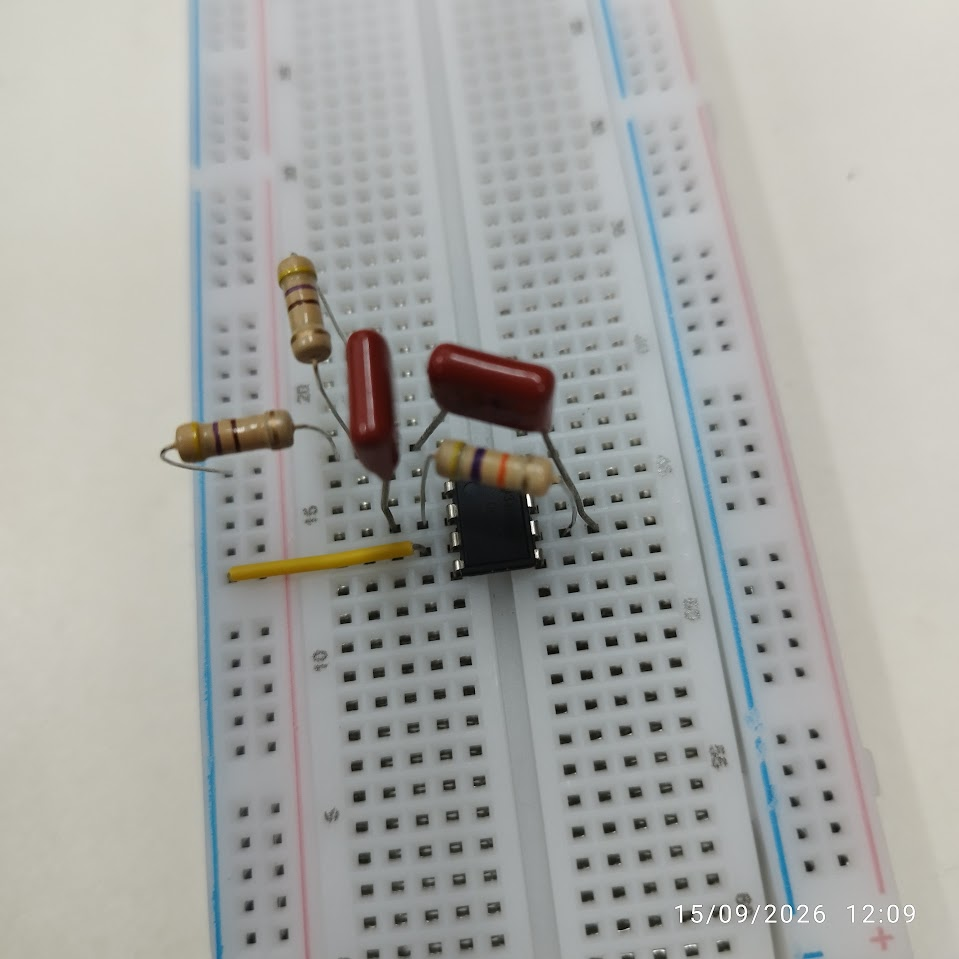
\includegraphics[
        trim=80bp 65bp 65bp 105bp,
        clip,
        width=\linewidth,
        height=0.43\textheight,
        keepaspectratio
      ]{prism-uploads/IMG_20260915_120903.jpg}

      \scriptsize Filtro MFB implementado em protoboard.
    \end{column}
    \hfill
    \begin{column}{0.31\textwidth}
      \centering
      \textbf{Baixa frequência: $40\,\mathrm{Hz}$}

      \vspace{0.08cm}
      \includegraphics[
        page=10,
        trim=150bp 503bp 126bp 145bp,
        clip,
        width=\linewidth,
        height=0.43\textheight,
        keepaspectratio
      ]{prism-uploads/cir02_pratica02_felipeppontes.pdf}

      \scriptsize Saída atenuada e defasagem próxima de $-90^\circ$.
    \end{column}
    \hfill
    \begin{column}{0.31\textwidth}
      \centering
      \textbf{Ressonância: $480\,\mathrm{Hz}$}

      \vspace{0.08cm}
      \includegraphics[
        page=10,
        trim=150bp 252bp 126bp 396bp,
        clip,
        width=\linewidth,
        height=0.43\textheight,
        keepaspectratio
      ]{prism-uploads/cir02_pratica02_felipeppontes.pdf}

      \scriptsize Maior ganho observado na vizinhança da frequência central.
    \end{column}
  \end{columns}

  \vspace{0.18cm}
  \centering\scriptsize Foto do circuito: acervo do autor. Osciloscópio: canal amarelo, saída $V_o$;
  canal verde, entrada $V_i$.
\end{frame}

\section{Discussão}
% Discussão dos resultados
\begin{frame}{Comparação entre teoria e experimento}
  \scriptsize
  \centering
  \begin{tabular}{rccccc}
    \toprule
    & \multicolumn{3}{c}{Magnitude} & \multicolumn{2}{c}{Fase ($^\circ$)} \\
    \cmidrule(lr){2-4}\cmidrule(lr){5-6}
    $f$ (Hz) & Teoria & Experimento & Erro & Teoria & Experimento \\
    \midrule
    40    & 0,5947  & 0,5674  & 4,59\%  & -90,68  & -91,0 \\
    100   & 1,5431  & 1,4995  & 2,83\%  & -91,77  & -90,0 \\
    400   & 18,1956 & 15,3616 & 15,58\% & -111,34 & -108,8 \\
    480,2 & 49,9733 & 42,4354 & 15,08\% & 178,13  & -153,5 \\
    1100  & 3,7874  & 4,0000  & 5,61\%  & 94,34   & 96,5 \\
    11000 & 0,3084  & 0,3486  & 13,03\% & 90,35   & 89,7 \\
    \bottomrule
  \end{tabular}

  \vspace{0.16cm}
  \begin{columns}[T,onlytextwidth]
    \begin{column}{0.48\textwidth}
      \begin{block}{Resultados confirmados}
        \begin{itemize}
          \item resposta passa-faixa preservada;
          \item ressonância experimental em $480{,}2\,\mathrm{Hz}$;
          \item boa concordância nas extremidades e na fase.
        \end{itemize}
      \end{block}
    \end{column}
    \begin{column}{0.48\textwidth}
      \begin{alertblock}{Principais fontes de desvio}
        \begin{itemize}
          \item tolerância de resistores e capacitores;
          \item produto ganho--banda do amplificador;
          \item parasitas da protoboard e ruído de medição;
          \item representação circular da fase junto à ressonância.
        \end{itemize}
      \end{alertblock}
    \end{column}
  \end{columns}
\end{frame}

\section{Conclusão}
% Conclusões da prática
\begin{frame}{Conclusões}
  \begin{itemize}
    \item A função de transferência descreveu corretamente a natureza passa-faixa do filtro MFB.
    \item O modelo previu uma frequência central de aproximadamente
      $478{,}9\,\mathrm{Hz}$ e ganho máximo próximo de 50.
    \item O LTspice reproduziu a ressonância e o comportamento global de magnitude e fase.
    \item A bancada apresentou pico em $480{,}2\,\mathrm{Hz}$, muito próximo do valor teórico.
    \item Os desvios de ganho são compatíveis com tolerâncias dos componentes e limitações do amplificador operacional real.
  \end{itemize}

  \begin{alertblock}{Síntese da prática}
    A integração entre análise, simulação e experimento permitiu validar o modelo e
    compreender os efeitos não ideais presentes no circuito físico.
  \end{alertblock}
\end{frame}

\section{Referências}
% Referências bibliográficas
\begingroup
\setbeamertemplate{bibliography item}[text]
\setbeamercolor{bibliography item}{fg=MalvaDestaque}
\setbeamercolor{bibliography entry author}{fg=RoxoPrincipal}
\setbeamercolor{bibliography entry title}{fg=CinzaTexto}
\setbeamercolor{bibliography entry location}{fg=RoxoSecundario}
\setbeamerfont{bibliography entry author}{series=\bfseries}
\setbeamertemplate{bibliography entry title}{\hspace{0.35em}}
\setbeamertemplate{bibliography entry location}{\hspace{0.35em}}
\setbeamertemplate{bibliography entry note}{\hspace{0.35em}}

\begin{frame}[t]{Referências bibliográficas}
  \vspace{0.04cm}
  \fontsize{7.4}{8.3}\selectfont
  \nocite{*}
  \bibliographystyle{plain}
  \bibliography{referencias}
\end{frame}
\endgroup

% Slide final
{
\setbeamercolor{background canvas}{bg=RoxoPrincipal}
\setbeamertemplate{footline}{}
\begin{frame}[plain]
  \begin{center}
    \vfill
    \marcaInstitucional{1.25cm}\par
    \vspace{0.55cm}
    {\color{white}\Huge\bfseries OBRIGADO}\par
    \vspace{0.4cm}
    {\color{MalvaDestaque}\rule{0.22\textwidth}{2pt}}\par
    \vspace{0.55cm}
    {\usebeamerfont{author}\color{white}\insertauthor\par}
    \vspace{0.18cm}
    {\usebeamerfont{institute}\color{white!84}\insertinstitute\par}
    \vspace{0.32cm}
    {\color{MalvaDestaque}\small\bfseries romariojonas.com\par}
    \vfill
  \end{center}
\end{frame}
}

\end{document}
